% Chapter 10

\chapter{Correction factors to the multiplicities} % Chapter title

\label{ch:CF} % For referencing the chapter elsewhere, use \autoref{ch:name}

%----------------------------------------------------------------------------------------

The \textit{raw} charged multiplicities presented in the previous chapter need to be corrected. The corrections discussed are acceptance correction i.e. the correction due to the geometrical limitation of the spectrometer and the data reconstruction efficiency, diffractive vector meson correction, radiative correction or electron contamination correction.

\section{Determination of the spectrometer acceptance} \label{sec:Acc}

\subsection{Monte Carlo sample from DJANGOH}

The COMPASS detector does not cover the full phase-space then the measured multiplicities have
to be corrected for the finite detector acceptance which is of the order of 70\%. The correction is
done using a Monte-Carlo dataset containing about 400 million events generated in the kinematic
region $Q^2 > 0.8$ (GeV/c)$^2$, $x$ $\in$ [10$^{-4}$,0.9], $y$ $\in$ [0.01,0.95], thanks to the Blue Waters facility computing power \cite{BLUEWATERS}. The kinematic region is larger than the one of interest in the analysis. This is done in order to be able to take into account smearing effects. These 400 millions events are divided in 4 different samples. As there is a difference in the experimental setup between the periods P07 and P08 onwards (two slabs in the OT), two different acceptance corrections should be applied. On the same basis, it was decided that the different beam charge should also have their own sample as there might be asymmetries in the spectrometer concerning the beam charge.

The events are created with DJANGOH generator with parametrization of the parton distribution functions (MSTW08). In addition, the use of JETSET inside DJANGOH allows the hadronization of quarks q to final-state hadrons h according to the Lund model. The COMPASS high $p_T$ tuning was used. The events of DJANGOH are then propagated into the experimental setup simulated by TGEANT. The output of this chain is referred to as \textit{generated} sample. These events are then reconstructed with the same CORAL code as used to reconstruct real data. This new sample is called \textit{reconstructed} sample. The same DIS event and unidentified hadron selection that are used on real data (except the BMS cut) are applied to the MC data sample for reconstructed MC events and particles.

The acceptance is calculated as the ratio of reconstructed over generated particles. In both cases, the particle ID is taken from the MC truth. The following selection is made on the generated particles :

\begin{enumerate}
  \item Energy of the beam muon in range [140,180] GeV
	\item Z coordinate of event vertex ($z_{vtx}$) within the target region $\in$ [-325 cm, -71 cm]
	\item Primary interaction in the target material (PHAST routine PaAlgo:InTarget() for both data and MC (Section \ref{sec:targetcut}) target positions to have a complete overlap of coverage)
	\item Beam track crossing the entire target (PHAST routine PaAlgo:CrossCells())
  \item $Q^2>1$ (GeV/c)$^2$
  \item $0.1 < y < 0.7$
	\item $5 < W < 17$ GeV/c$^2$
  \item $0.004 < x < 0.4$
  \item $\nu$ range used in data
  \item $0.2 < z < 0.85$
\end{enumerate}

The inclusive kinematic variables $Q^2$, $x$ and $y$ and semi-inclusive variables $z$ and $p_h$ are shown in Figs. \ref{pic:MCDISkin} and \ref{pic:MCSIDISkin} for real (red) and reconstructed MC data (blue). The ratio between real and reconstructed MC data is plotted in each bottom panel. A relative good agreement is reached, except in the high $x$ and high $Q^2$ regions. This discrepancy should not be too much of a problem as in the multiplicities, the inclusive acceptance is cancelling by and large.

\begin{figure}[!h]
	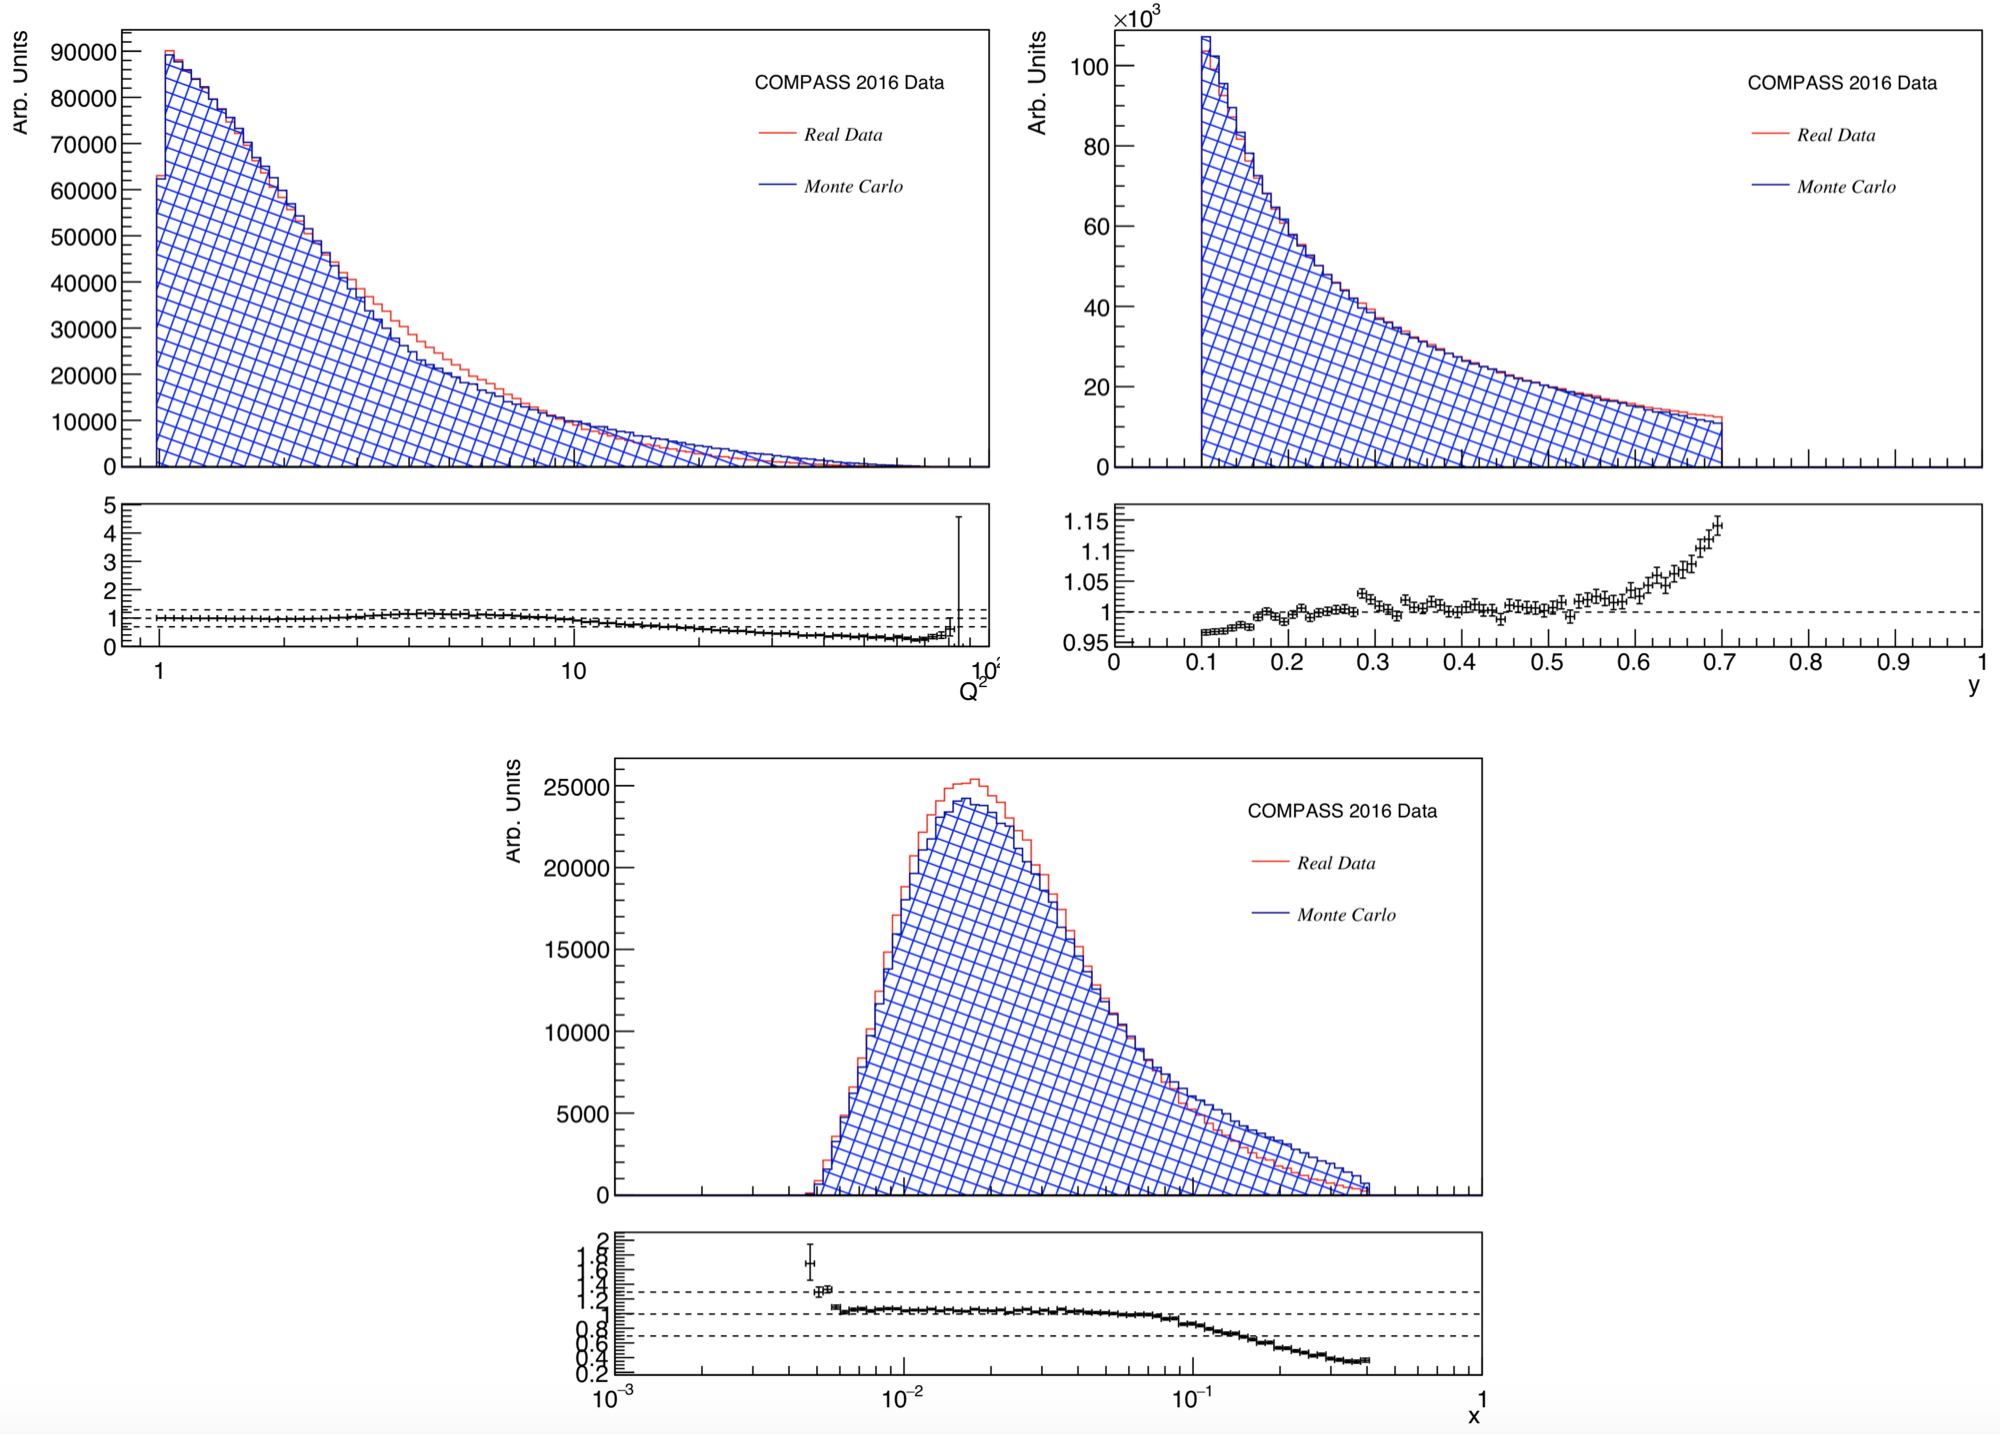
\includegraphics[scale=0.45]{./gfx/DIS_kin.png}
	\caption{Kinematical variables for DIS events ($Q^2$, $y$ and $x$) for Data (red) and Monte-Carlo (blue), as well as the ratio Data/Monte-Carlo.}
	\label{pic:MCDISkin}
\end{figure}

\begin{figure}[!h]
	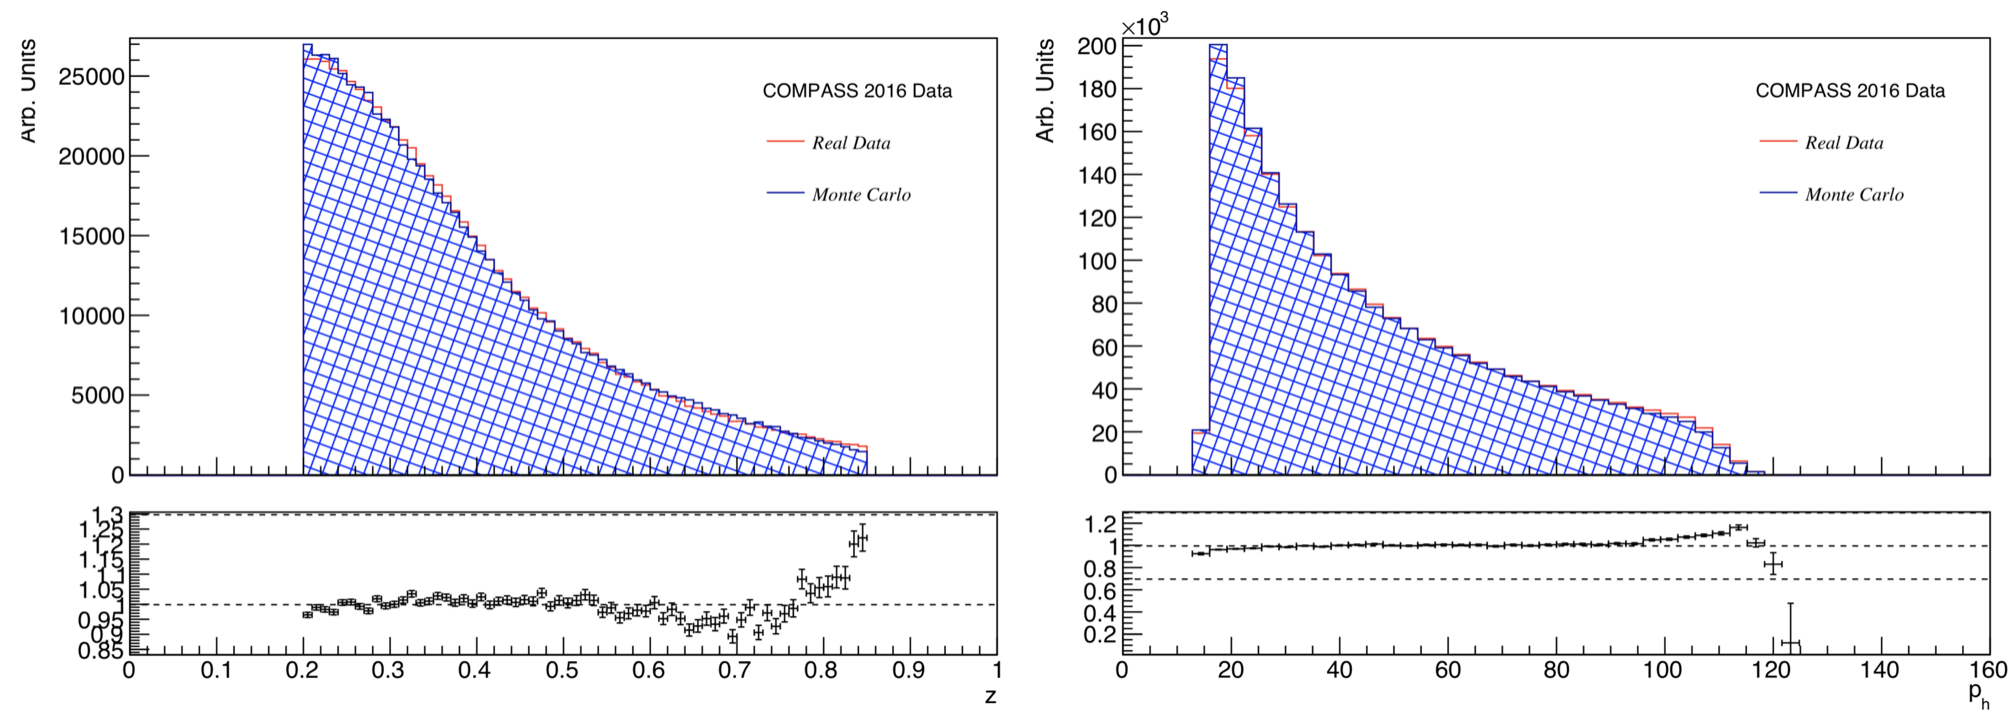
\includegraphics[scale=0.45]{./gfx/SIDIS_kin.png}
	\caption{Kinematical variables for charged hadrons ($z$ and $p_h$) for Data (red) and Monte-Carlo (blue), as well as the ratio Data/Monte-Carlo.}
	\label{pic:MCSIDISkin}
\end{figure}

\subsection{Acceptance calculation}

In the following, $r$ and $g$ refers to 'reconstructed' and 'generated' quantities.

The acceptance is determined as the ratio of reconstructed multiplicities $M^h_r$ over the generated multiplicities $M^h_g$ and is binned in $x$, $y$ and $z$ :

\begin{equation}
  A^h(x,y,z) = \frac{M^h_r(x,y,z)}{M^h_g(x,y,z)}=\frac{N^h_r(x,y,z)/N^{DIS}_r(x,y,z)}{N^h_g(x,y,z)/N^{DIS}_g(x,y,z)}
\end{equation}

where $x_g$, $y_g$ and $z_g$ are the generated kinematic values and $x_r$, $y_r$ and $z_r$ are the reconstructed kinematic values.

The acceptance correction factors $A^h(x,y,z)$ for unidentified hadrons, pions, kaons and protons are shown in Figs. \ref{pic:AccH} to \ref{pic:AccP} for the P07 sample. Note that the acceptance is very similar for positive and negative particles and for $\mu^+$ and $\mu^-$ beams.

\begin{sidewaysfigure}[!]
  \centering
	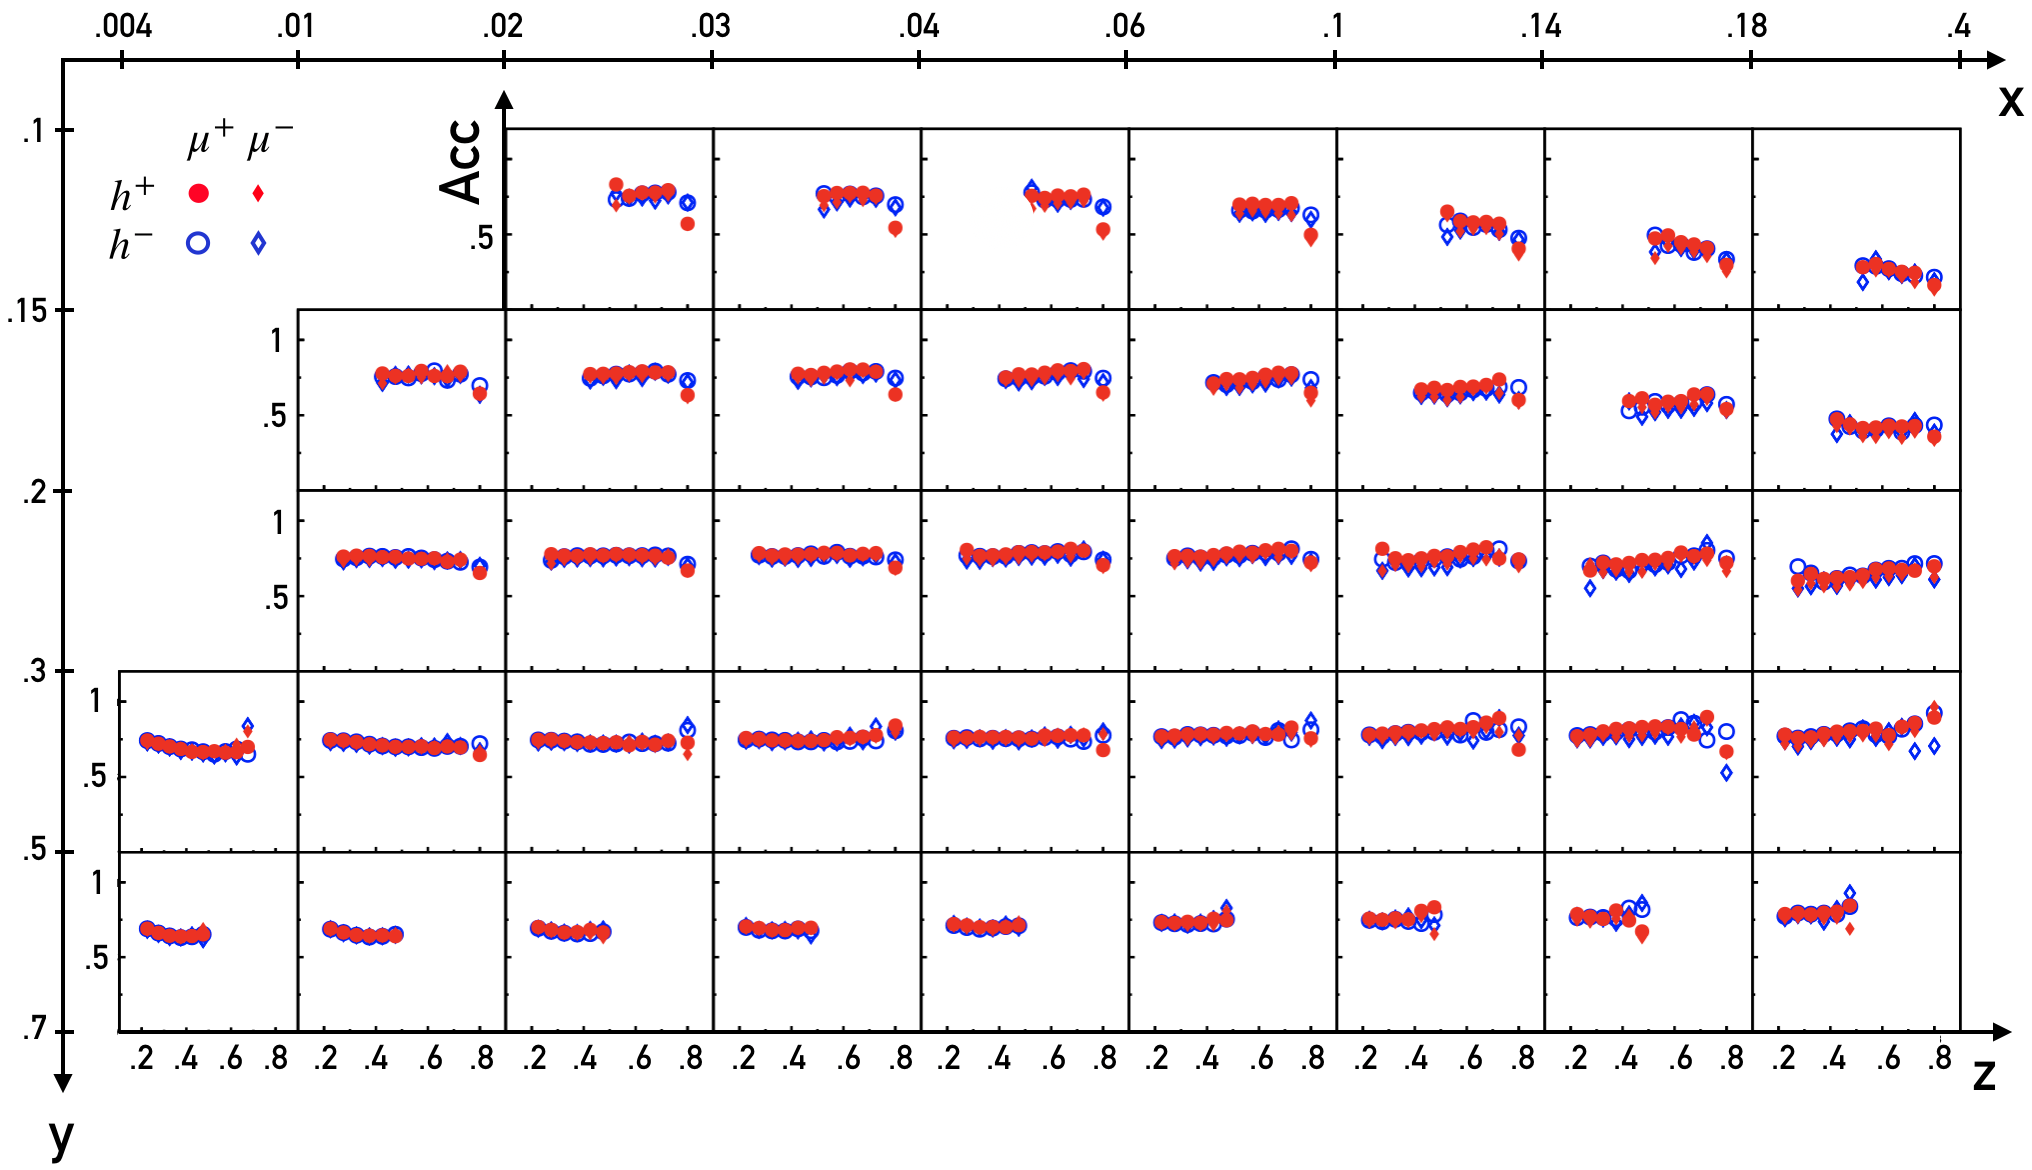
\includegraphics[scale=0.6]{./gfx/AccH.png}
	\caption{Charged hadron acceptance in $x$, $y$ and $z$ bins. The red full markers correspond to positive hadrons, blue open markers to negative hadrons, circles markers correspond to hadrons obtained with $\mu^+$ beam and diamonds markers to hadrons obtained with $\mu^-$ beam.}
	\label{pic:AccH}
\end{sidewaysfigure}

\begin{sidewaysfigure}[p]
  \centering
	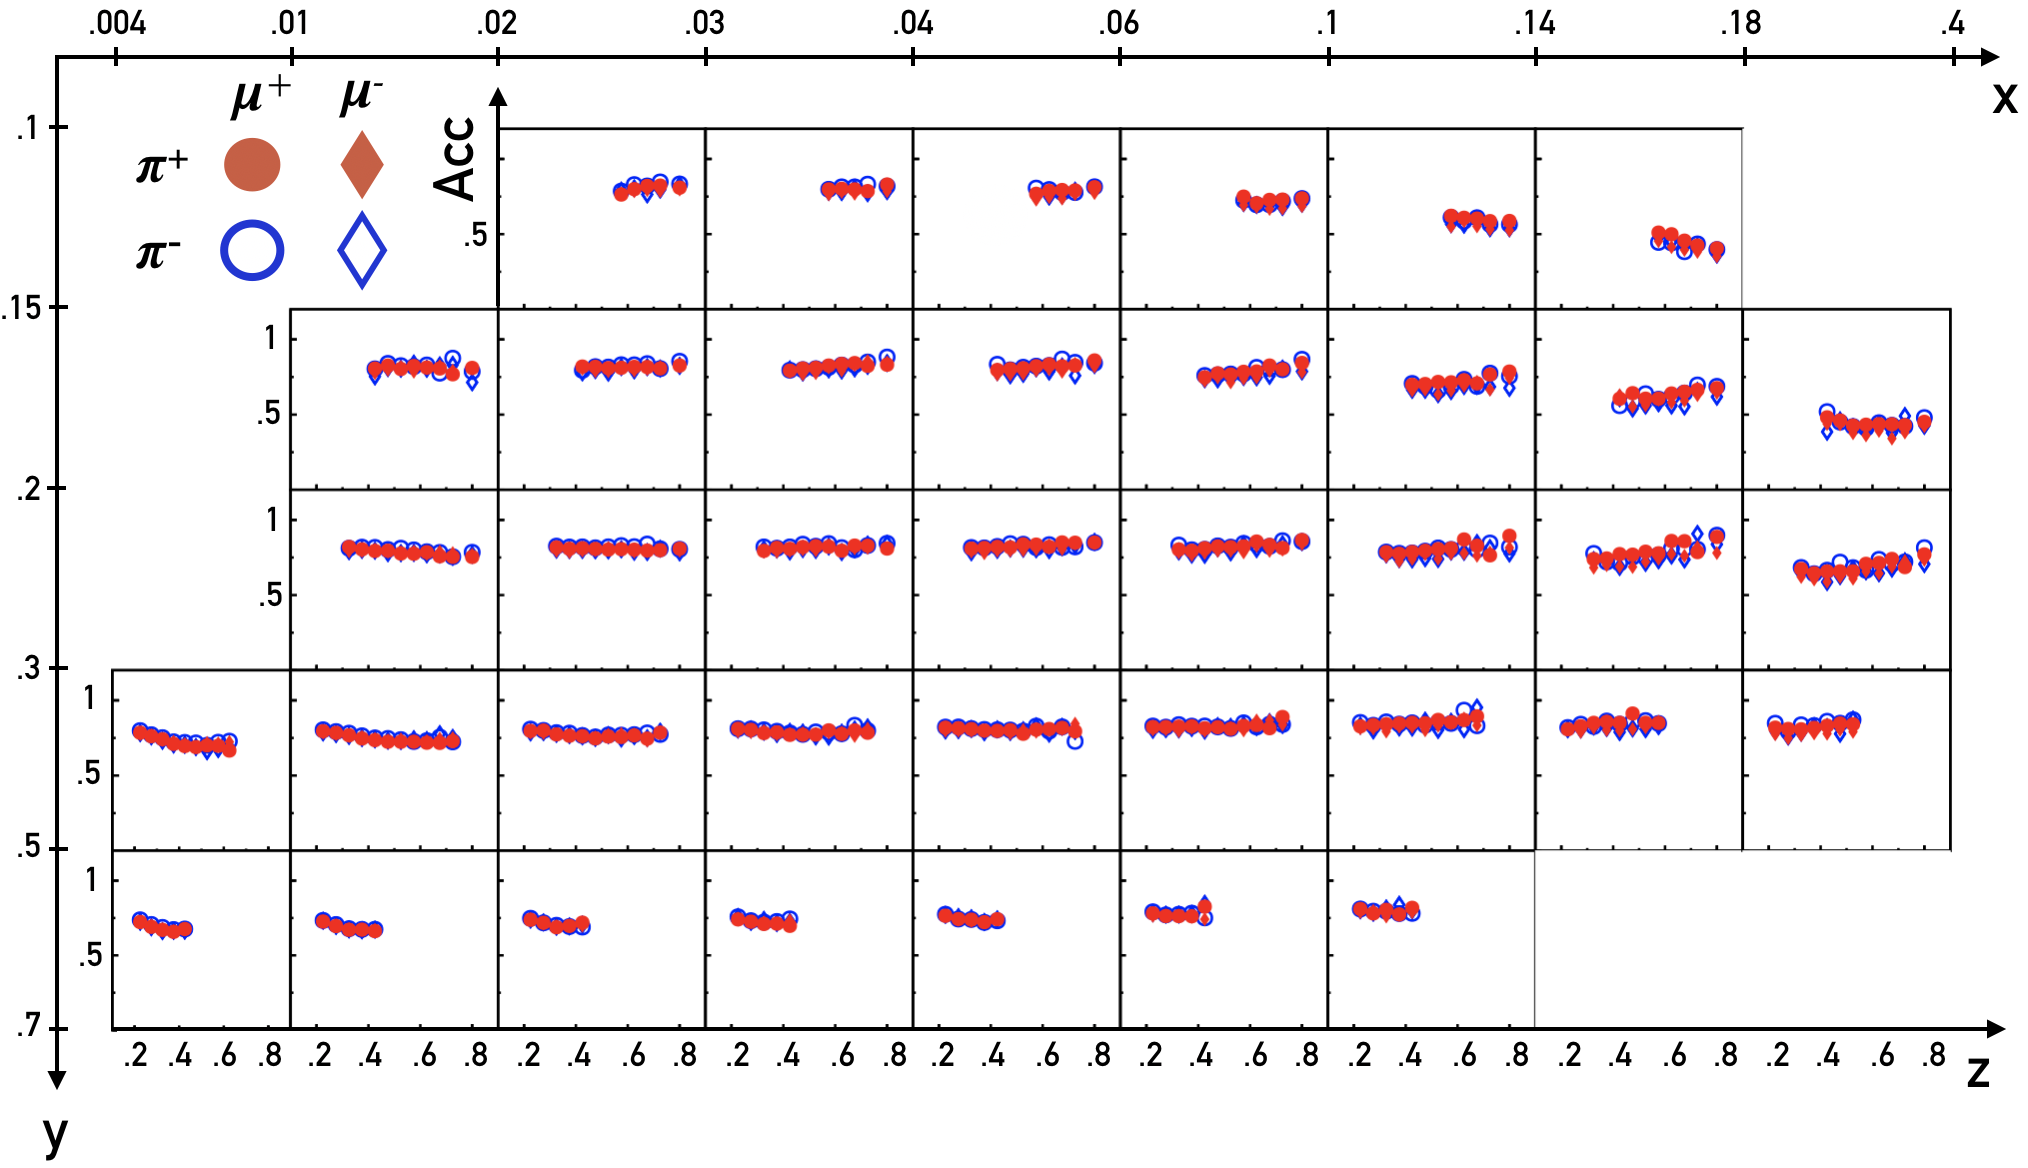
\includegraphics[scale=0.6]{./gfx/AccPi.png}
	\caption{Charged pion acceptance in $x$, $y$ and $z$ bins. The red full markers correspond to positive hadrons, blue open markers to negative hadrons, circles markers correspond to pions obtained with $\mu^+$ beam and diamonds markers to hadrons obtained with $\mu^-$ beam.}
	\label{pic:AccPi}
\end{sidewaysfigure}

\begin{sidewaysfigure}[p]
  \centering
	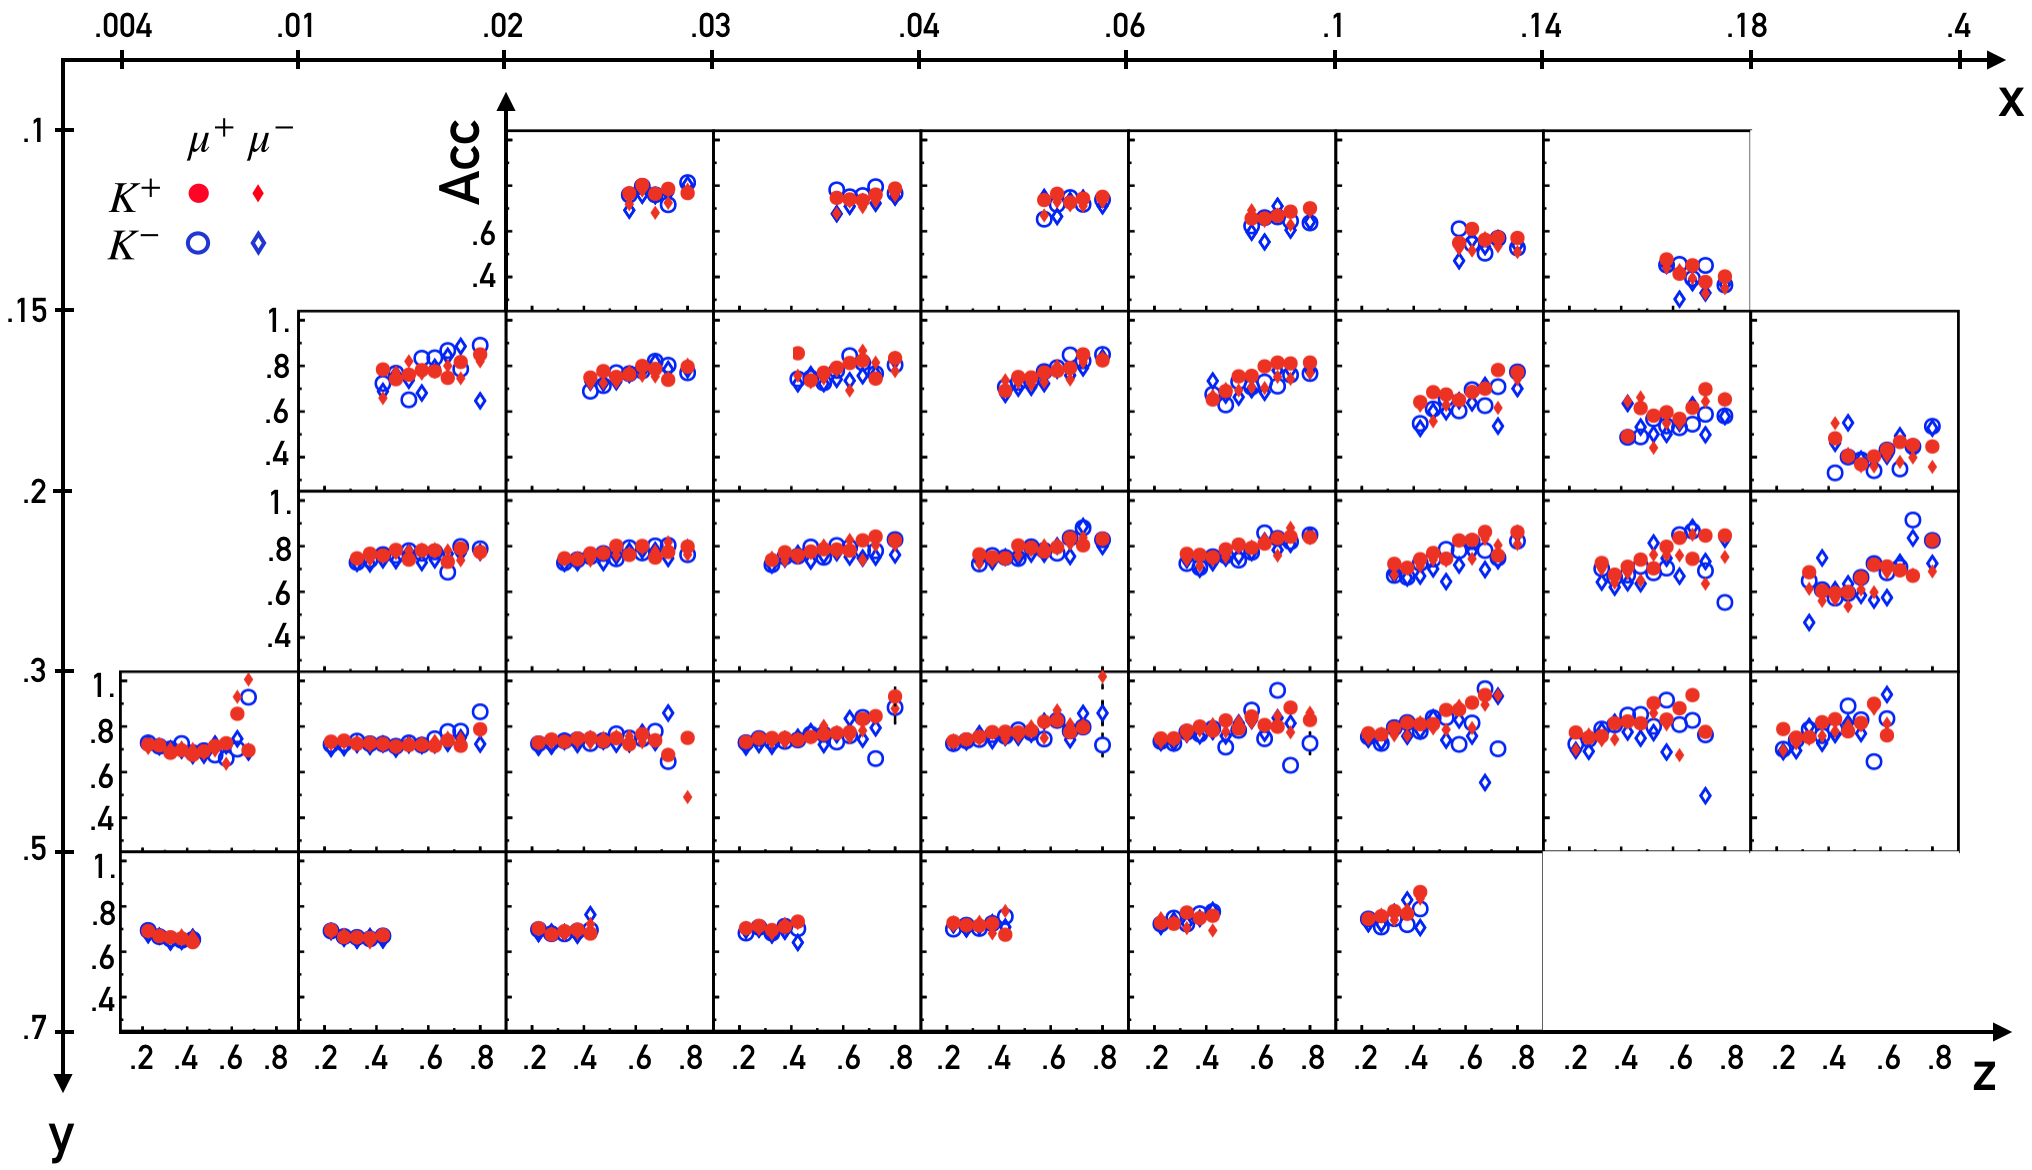
\includegraphics[scale=0.6]{./gfx/AccK.png}
	\caption{Charged kaon acceptance in $x$, $y$ and $z$ bins. The red full markers correspond to positive hadrons, blue open markers to negative hadrons, circles markers correspond to kaons obtained with $\mu^+$ beam and diamonds markers to hadrons obtained with $\mu^-$ beam.}
	\label{pic:AccK}
\end{sidewaysfigure}

\begin{sidewaysfigure}[p]
  \centering
	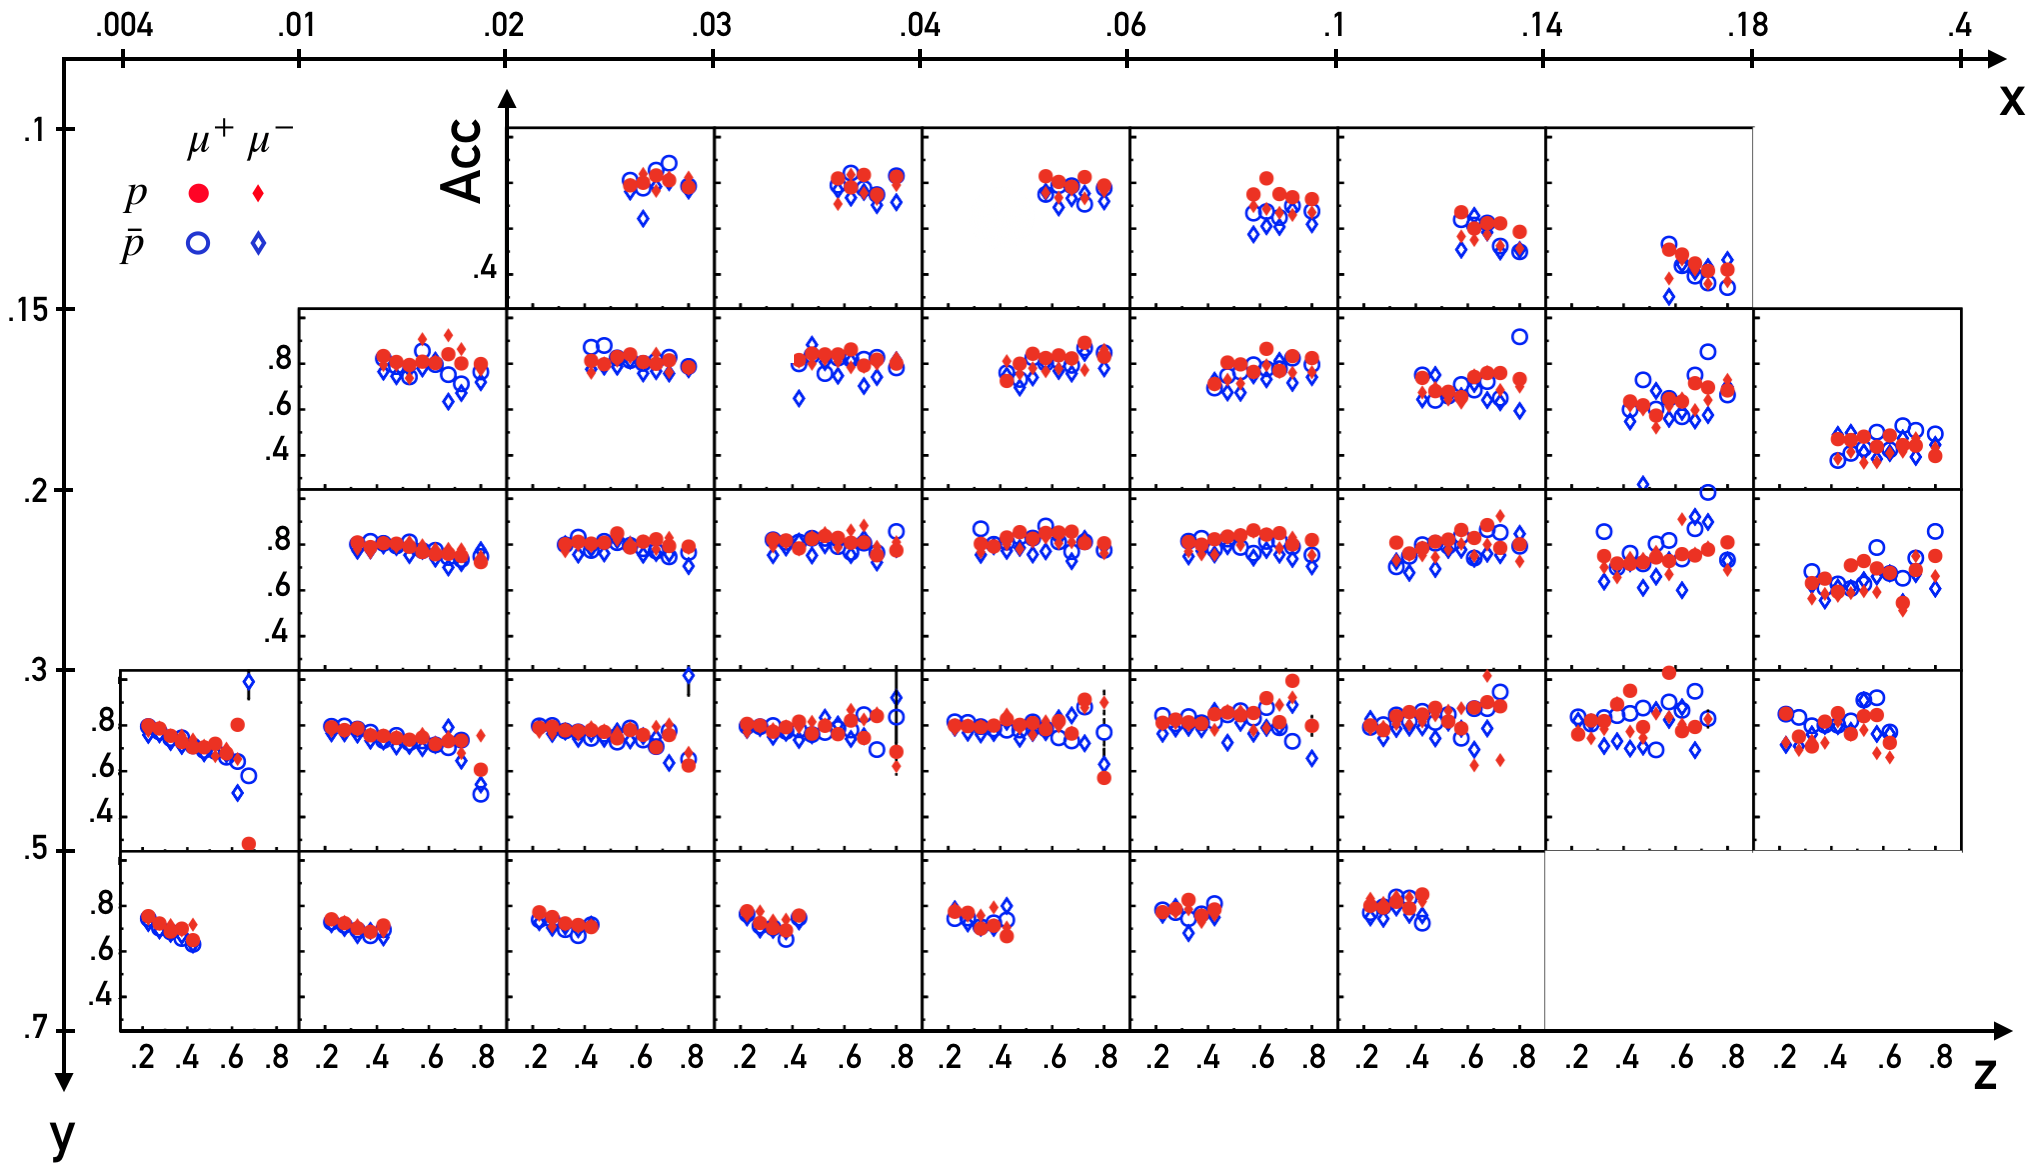
\includegraphics[scale=0.5]{./gfx/AccP.png}
	\caption{Charged proton acceptance in $x$, $y$ and $z$ bins. The red full markers correspond to positive hadrons, blue open markers to negative hadrons, circles markers correspond to kaons obtained with $\mu^+$ beam and diamonds markers to hadrons obtained with $\mu^-$ beam.}
	\label{pic:AccP}
\end{sidewaysfigure}

In Fig. \ref{pic:AccPer} are compared the acceptance correction factors for the P07 and P09 samples. The discrepancy is only visible in the highest $x$ bins.

\begin{sidewaysfigure}[p]
  \centering
	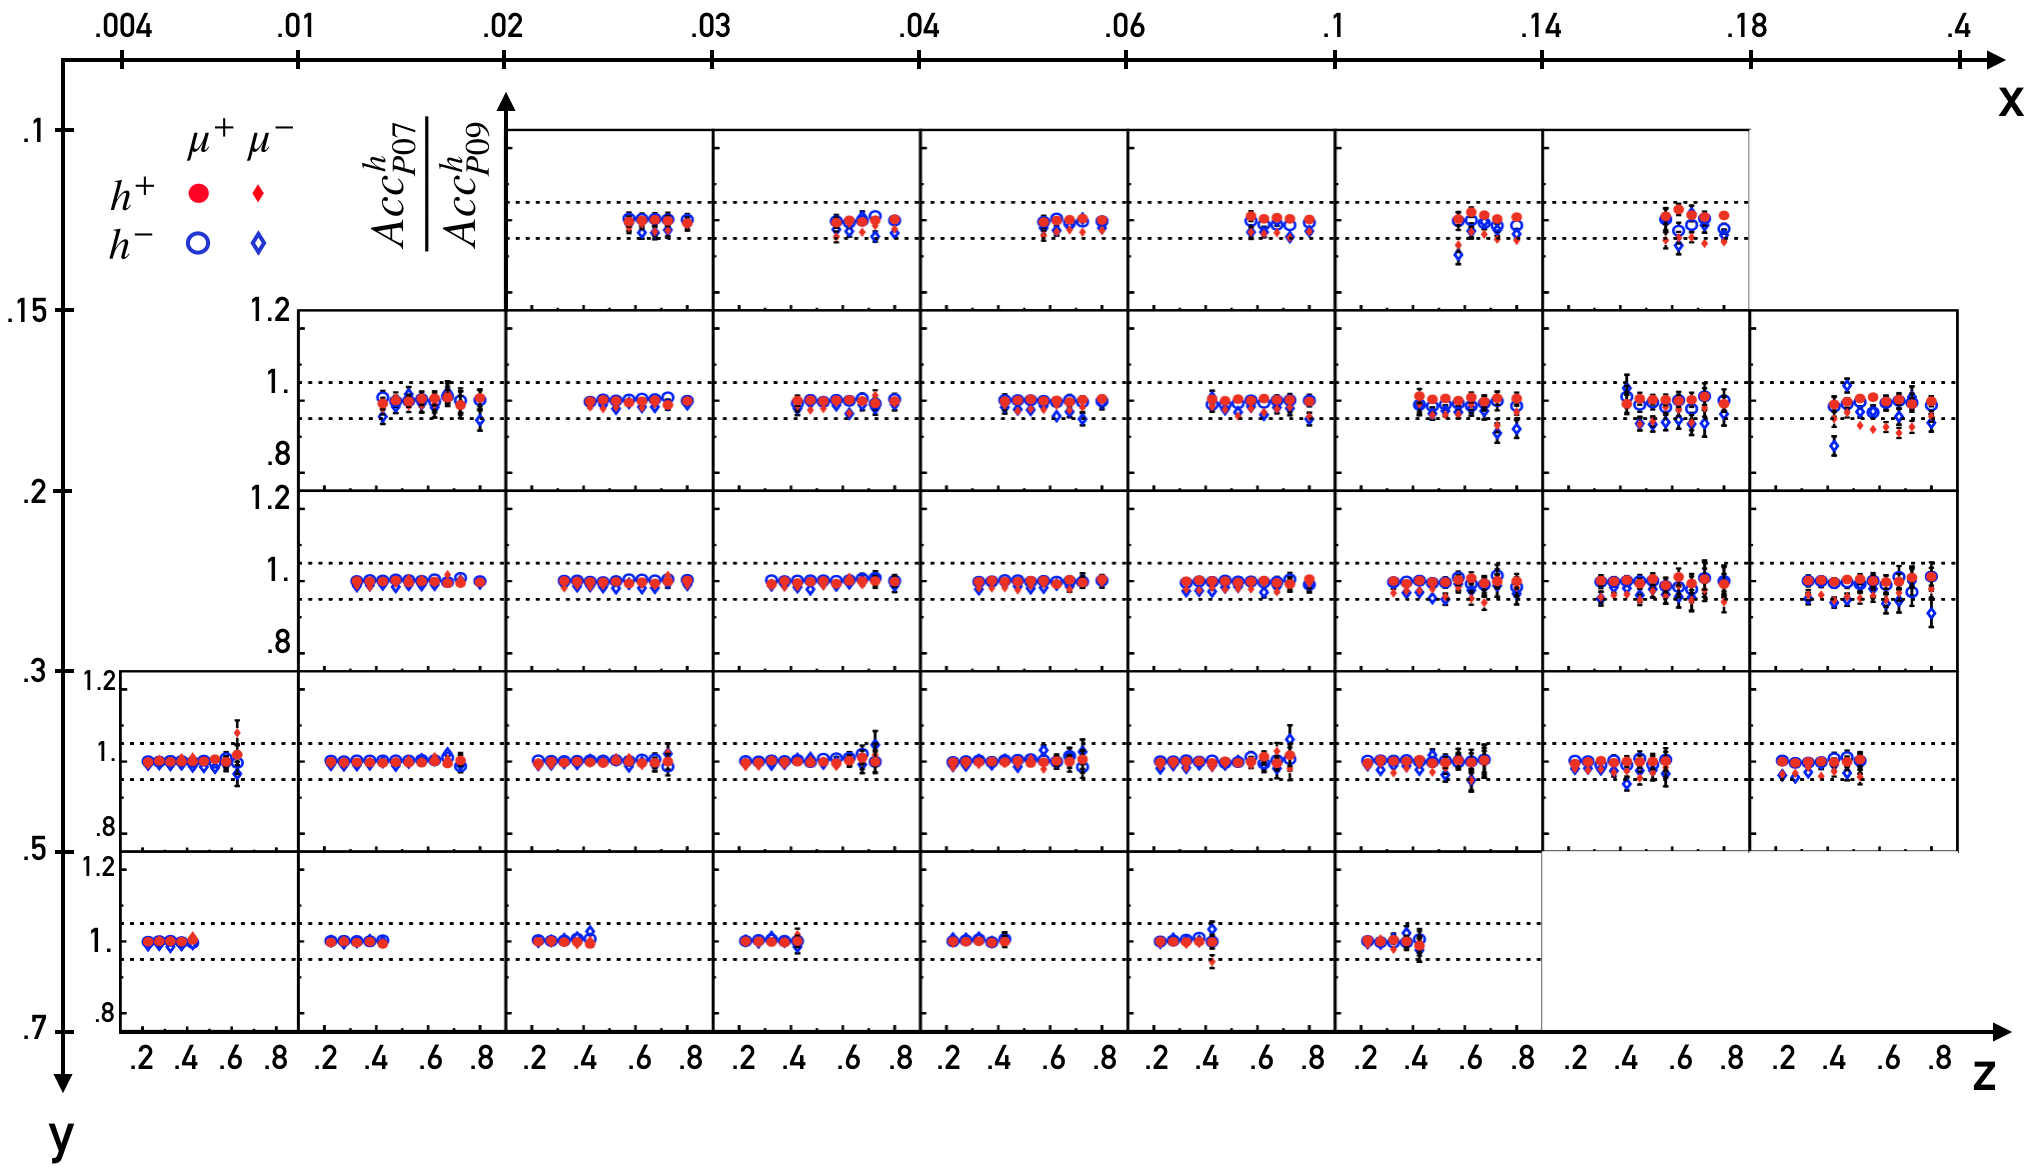
\includegraphics[scale=0.6]{./gfx/SysAcc.png}
	\caption{Ratio of P07 over P09 acceptance in $x$, $y$ and $z$ bins. The dashed lines represent a 5\% discrepancy.}
	\label{pic:AccPer}
\end{sidewaysfigure}

Used in this fashion, the kinematic bin smearing due to reconstruction limitations is accounted for. A more rigorous bin smearing correction would involve an unfolding procedure but is not done in this analysis.

For this method, the error estimation is difficult to rigorously calculate as the numbers of evaluated hadrons and DIS events, in both the reconstructed and generated case, are not independent. An estimation is made by considering that the hadron numbers and DIS events are independent of each other. Due to the $z$ kinematic bin migration effects, there exist particles in $N_r$ which are independent from $N_g$. Decomposing $N_r$ into two independent samples namely $N_{r^0}$ which are contained in $N_g$ and $N_{r'}$ which are not, the final acceptance error yields :

\begin{equation}
  \begin{split}
    E^2_{acc} = \left (\frac{G_D}{R_D+R'_{D}}\right )^2\left [\frac{(R_h+A)(G_h-R_h+1)}{(G_h+2)^2(G_D+3)}+\frac{R'_{h}}{G^2_h}+\frac{R'^2_h}{G^3_h}\right ] \\
                + \left (\frac{G_D}{R_D+R'_{D}}\right )^4\left (\frac{R_h+R'_h}{G_h}\right )^2\left [\frac{(R_D+1)(G_D-R_D+1)}{(G_D+2)^2(G_D+3)}+\frac{R'_D}{G^2_D}+\frac{R'^2_D}{G^3_D}\right ]
  \end{split}
\end{equation}

where $G_h$ (resp. $G_D$) are the generated hadrons (resp. DIS events) in a given $x$, $y$, $z$ bin, $R_h$ (resp. $R_D$) the reconstructed hadrons (resp. DIS events) and $R'_h$ (resp. $R'_D$) all other particles (resp. events) that are reconstructed as hadrons (resp. DIS events) in a given $x$, $y$, $z$ bin.

The correction is then applied to the raw multiplcities :

\begin{equation}
  M^h(x,y,z) = \frac{M^h_{raw}(x,y,z)}{A^h(x,y,z)}
\end{equation}

\newpage

\section{Diffractive vector meson correction} \label{sec:DVMf}

It is usually assumed that hadrons produced in SIDIS originate from lepton-parton scattering. Nevertheless the scattering of a lepton off a nucleon can also result in the diffractive production of vector mesons. These particles decay into lighter mesons that cannot be distinguished from the one resulting from the hadronization of a quark originating from the target nucleon. This implies that fragmentation functions extracted from multiplicities contaminated with diffractive vector mesons would violate universality, as they would be process dependent. However, this is a complex theoretical discussion so the multiplicities both with and without subtracting the diffractive vector meson contribution are calculated as well as the separate correction factors for DIS events and hadrons.

For pions and kaons, the dominant vector meson contribution comes from the diffractive production of $\rho^0$ and $\Phi$, respectively :

\begin{equation}
    \begin{split}
      \gamma * p \rightarrow \rho^0 p \rightarrow p\pi^+\pi^- \\
      \gamma * p \rightarrow \Phi p \rightarrow pK^+K^-
    \end{split}
\end{equation}

\begin{figure}[!h]
  \centering

  \subfloat[]{\begin{tikzpicture} \begin{feynman}
\vertex (i1) {\(l\)};
\vertex[below right=2cm of i1] (a);
\vertex[above right=2cm of a] (i2) {\(l'\)};
\vertex[below=2cm of a] (b);
\vertex[below=2cm of b] (c) {\(V\)};
\vertex[dot, below=1cm of b] (e);
\vertex[left=3cm of e] (d);
\vertex[blob, below=2cm of c] (g) {};
\vertex[above right=2cm of g] (f1) {\(\pi^+,K^+\)};
\vertex[below right=2cm of g] (f2) {\(\pi^-,K^-\)};
\vertex[above=2cm of d] (n1) {\(N\)};
\vertex[below=2cm of d] (n2) {\(N\)};


\diagram* { (i1) -- [fermion] (a) -- [fermion] (i2),
(a) -- [photon, edge label=\(\gamma^*\)] (b),
(n1) -- [double distance=7pt] (d) -- [double distance=7pt] (n2),
(n1) -- [fermion] (d) -- [fermion] (n2),
(b) -- [fermion, half left, looseness=1.5, edge label=\(q\)] (c),
(b) -- [anti fermion, half right, looseness=1.5, edge label=\(\bar{q}\)] (c),
(d)-- [plain, half left, looseness=1.5] (e),
(d)-- [plain, half right, looseness=1.5] (e),
(c) -- [double distance=7pt] (g) [blob],
(g) [blob] -- [double distance=7pt] (f1),
(g) [blob] -- [double distance=7pt] (f2),
};
\end{feynman} \end{tikzpicture}}
\hspace{2cm}
\subfloat[]{\begin{tikzpicture} \begin{feynman}
\vertex (i1) {\(l\)};
\vertex[below right=2cm of i1] (a);
\vertex[above right=2cm of a] (i2) {\(l'\)};
\vertex[dot, below=2cm of a] (b);
\vertex[below=2cm of b] (c) {\(V\)};
\vertex[below=1cm of b] (e);
\vertex[left=3cm of e] (d);
\vertex[blob, below=2cm of c] (g) {};
\vertex[above right=2cm of g] (f1) {\(\pi^+,K^+\)};
\vertex[below right=2cm of g] (f2) {\(\pi^-,K^-\)};
\vertex[above=2cm of d] (n1) {\(N\)};
\vertex[below=2cm of d] (n2) {\(X\)};


\diagram* { (i1) -- [fermion] (a) -- [fermion] (i2),
(a) -- [photon, edge label=\(\gamma^*\)] (b),
(n1) -- [double distance=7pt] (d) -- [double distance=7pt] (n2),
(n1) -- [fermion] (d) -- [plain] (n2),
(b) -- [fermion, half left, looseness=1.5, edge label=\(q\)] (c),
(b) -- [anti fermion, half right, looseness=1.5, edge label=\(\bar{q}\)] (c),
(d) -- [plain, half left, looseness=1.5] (e),
(d) -- [plain, half right, looseness=1.5] (e),
(c) -- [double distance=7pt] (g) [blob],
(g) [blob] -- [double distance=7pt] (f1),
(g) [blob] -- [double distance=7pt] (f2),
};
\end{feynman} \end{tikzpicture}}
	\caption{Vector meson diffractive production (V in the figure, being $\rho^0$, $\Phi$, etc..). In the VMD model\cite{VMD}, the $\gamma^*$ virtual photon creates a $q\bar{q}$ pair with compatible quantum numbers. Two cases can be encountered : vector meson exclusive production (where the same nucleon is found in the final state) (a) and vector meson production with nucleon diffractive dissociation (b).}
	\label{pic:DVMprod}
\end{figure}

This process is mainly exclusive but in 20\% of cases a diffractive dissociation of the target nucleon occurs. Other channels (excited $\rho$, $\omega$, etc.) are expected to contribute much less and are not taken into account. As pions and kaons stemming from diffractive vector meson decay cannot be separated from the one resulting from SIDIS, the evaluation of their contribution to the multiplicities is based on a Monte Carlo study. Three Monte Carlo samples are produced based on different generators (SIDIS using DJANGOH, diffractive $\Phi$ using HEPGEN++) and the same event reconstruction chain. For the diffractive vector meson samples, both exclusive events and events with diffractive dissociation of the proton are simulated. The $\rho^0$ sample includes nuclear effects (coherent production and nuclear absorption).

The fraction of pions (resp. kaons) resulting from a diffractive $\rho^0$ (resp. $\Phi$) is calculated in the same binning as the raw multiplicities as :

\begin{equation}
  \begin{split}
    f^{\pi}_{\rho^0}(x,y,z) = \frac{N^{\pi}_{HEPGEN++}(x,y,z)}{N^{\pi}_{DJANGOH}(x,y,z)+N^{\pi}_{HEPGEN++}(x,y,z)} \\
    f^K_{\Phi}(x,y,z) = \frac{N^K_{HEPGEN++}(x,y,z)}{N^K_{DJANGOH}(x,y,z)+N^K_{HEPGEN++}(x,y,z)}
  \end{split}
\end{equation}

where $N^{\pi}_{HEPGEN++}$, $N^{\pi}_{DJANGOH}$, $N^K_{HEPGEN++}$ and $N^K_{DJANGOH}$ are the number of kaons reconstructed from the HEPGEN++ and DJANGOH MC samples normalized by the corresponding MC luminosity ($L_{MC}$). The luminosity depends on the event weighting and the process cross-section $\sigma_{int}$, as shown in Fig. \ref{eq:reweight} (DIS for DJANGOH event and diffractive vector meson production for HEPGEN++ events). The final weighted number of DIS events and hadrons is summarized in Table \ref{DVM}.

\begin{equation} \label{eq:reweight}
  \sum_{events} w_i = L_{MC} \cdot \sigma{int}
\end{equation}

\begin{table}
	\centering
	\begin{tabular}{rccc}
    \hline
     & DJANGOH & $\rho^0$ & $\Phi$ \\
    \hline
    Generated Events & 8.4M & 19.1M & 19.2M  \\
    Weighted Generated Events & 8.4M & 280.2M & 576.9M  \\
		Integrated Cross-Section [pb] & 227010 & 12200 & 2500  \\
		Monte-Carlo Luminosity [pb$^-1$] & 36.8 & 22966.6 & 23075.2  \\
    \hline
		DIS Events [pb] & 3.4M & 96209.4 & 18083.2  \\
		$h^+$ [pb] & 630880 & 25301.9 & 3890.26  \\
		$h^-$ [pb] & 511014 & 25250.4 & 4033.93  \\
		$\pi^+$ [pb] & 453794 & 25257.4 & -  \\
		$\pi^-$ [pb] & 377335 & 25212.3 & -  \\
		$K^+$ [pb] & 102019 & - & 3872.66  \\
		$K^-$ [pb] & 75158 & - & 4015.85 \\
  \end{tabular}
  \caption{Weighted number of DIS events and hadrons for the diffractive vector meson correction.}
  \label{DVM}
\end{table}

The diffractive vector meson events can also lead to a contamination in DIS events. Here, the two channels studied are diffractive $\rho^0$ and $\Phi$ with the fraction of the contamination expressed in Eqs. 13. Contrary to previous Eq. 11, the denominator only includes the DIS events from the DJANGOH generator because the cross-section used to generate the DJANGOH sample takes into account the diffractive contribution.

\begin{sidewaysfigure}[!]
  \centering
	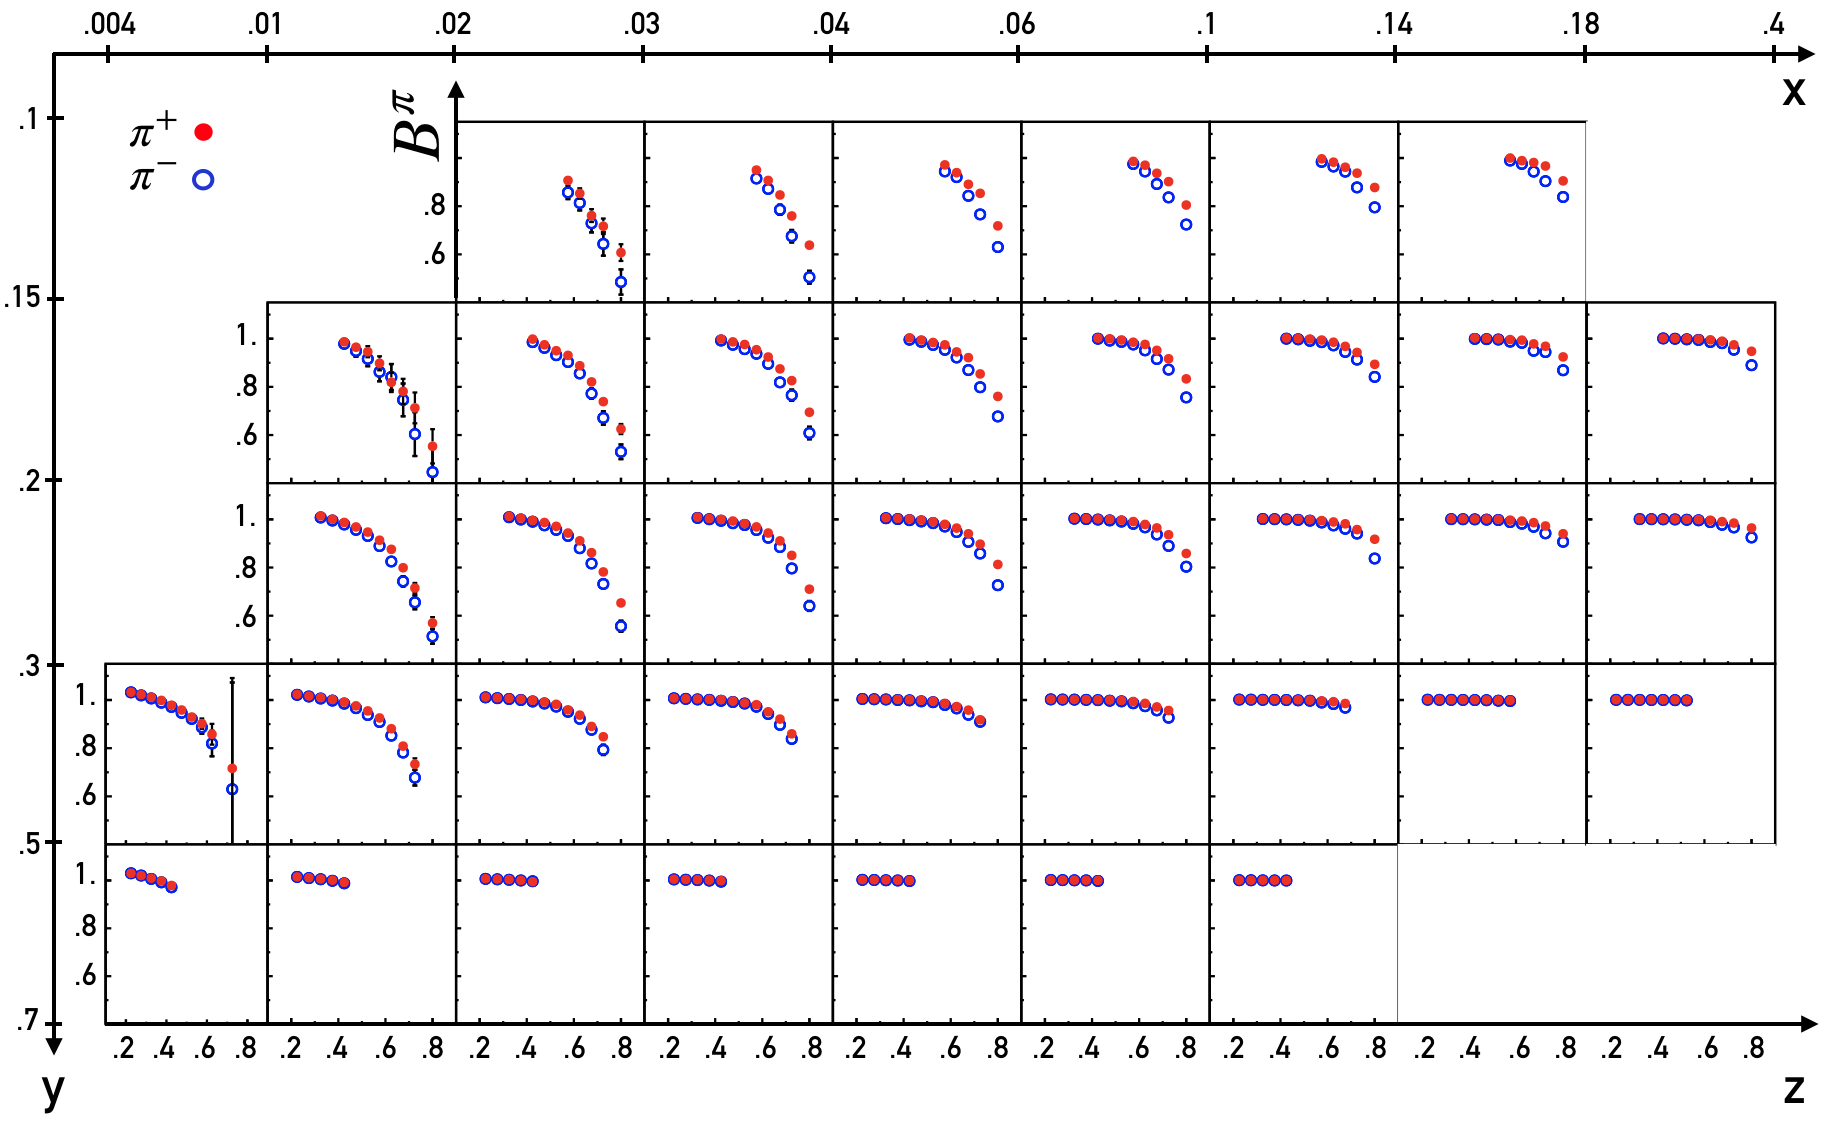
\includegraphics[scale=0.5]{./gfx/DVMpi.png}
	\caption{Correction factor $B^{\pi}$ for diffractive vector meson contamination ($\rho^0$) as a function of $z$ for ($x$,$y$) bins. The red markers correspond to positive pions and blue markers for negative pions.}
	\label{DVMpi}
\end{sidewaysfigure}

\begin{sidewaysfigure}[!]
  \centering
	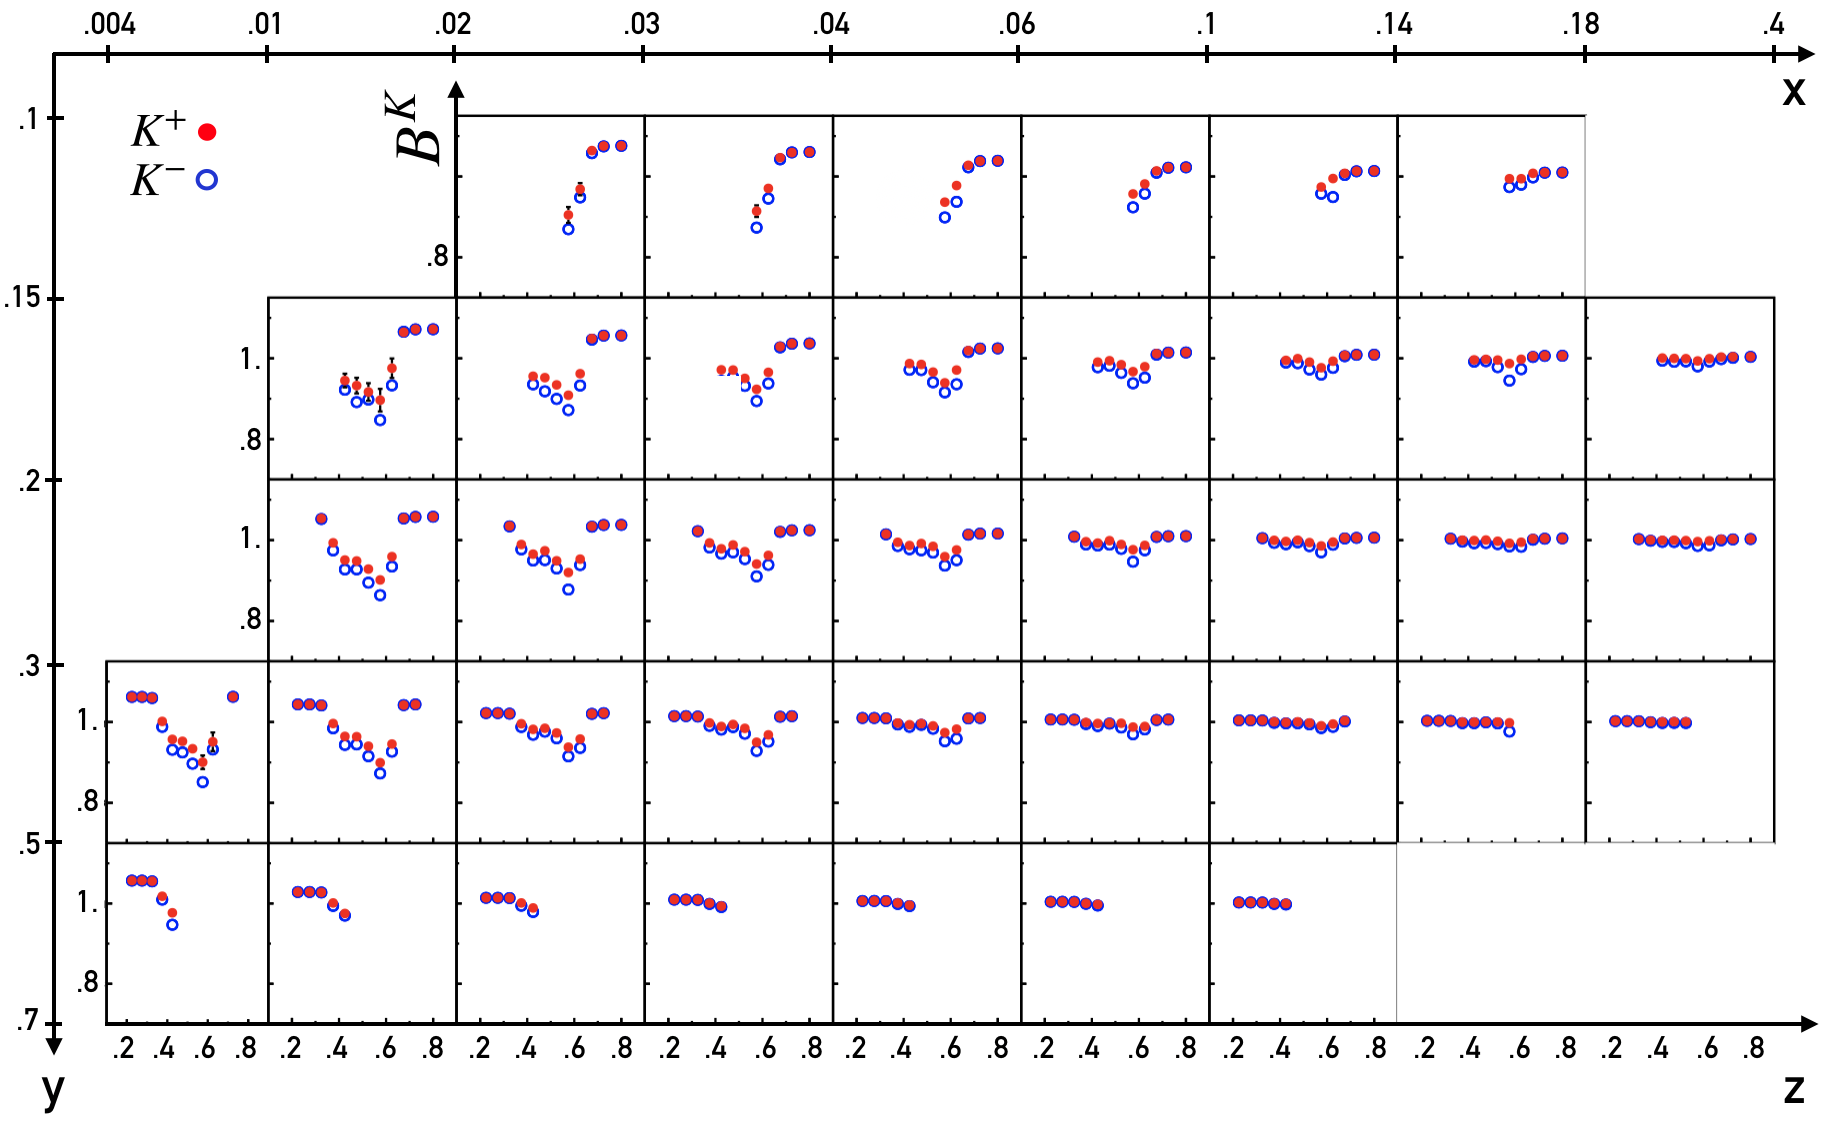
\includegraphics[scale=0.7]{./gfx/DVMK.png}
	\caption{Correction factor $B^{K}$ for diffractive vector meson contamination ($\Phi$) as a function of $z$ for ($x$,$y$) bins. The red markers correspond to positive kaons and blue markers for negative kaons.}
	\label{DVMK}
\end{sidewaysfigure}

\begin{equation}
  \begin{split}
    f^{\rho^0}_{DIS}(x,y,z) = \frac{N^{DIS}_{\rho^0,HEPGEN++}(x,y,z)}{N^{DIS}_{DJANGOH}(x,y,z)+N^{DIS}_{\rho^0,HEPGEN++}(x,y,z)+N^{DIS}_{\Phi,HEPGEN++}(x,y,z)} \\
    f^{\Phi}_{DIS}(x,y,z) = \frac{N^{DIS}_{\Phi,HEPGEN++}(x,y,z)}{N^{DIS}_{DJANGOH}(x,y,z)+N^{DIS}_{\rho^0,HEPGEN++}(x,y,z)+N^{DIS}_{\Phi,HEPGEN++}(x,y,z)}
  \end{split}
\end{equation}

The total contribution from the diffractive vector-meson contribution ($f^{VM}_{DIS}$) to the DIS sample is the sum of the $f^{\rho^0}_{DIS}$ and $f^{\Phi}_{DIS}$. The final correction reads as follows :

\begin{equation}
  \begin{split}
  B^h(x,y,z) = \frac{ \frac{N^{\pi}(x,y,z)}{N^h(x,y,z)}\left (1-f^{\pi}_{\rho^0}(x,y,z)\right )
                   + \frac{N^K(x,y,z)}{N^h(x,y,z)}\left (1-f^{K}_{\Phi}(x,y,z)\right ) + \frac{N^p(x,y,z)}{N^h(x,y,z)} }{1-f^{VM}_{DIS}(x,y,z)} \\
  B^{\pi}(x,y,z) = \frac{1-f^{\pi}_{\rho^0}(x,y,z)}{1-f^{VM}_{DIS}(x,y,z)} \\
  B^K(x,y,z) = \frac{1-f^{K}_{\Phi}(x,y,z)}{1-f^{VM}_{DIS}(x,y,z)}
  \end{split}
\end{equation}

The correction for pions has the strongest impact at high $z$ ($z>0.5$) and low $x$ ($x<0.02$) where it can reach 50\%, while the correction for kaons has the strongest impact at middle $z$ ($0.4<z<0.6$) and low $x$ ($x<0.02$) where it can reach 20\%.

\section{Radiative corrections} \label{sec:rcf}

The experimental multiplicities are affected by QED radiative effects, which introduce a systematic bias of the measured kinematics with respect to the true kinematics. The most important contributions at first order are the initial and final state radiation of a real photon by the incoming or outgoing lepton. The correction factor used to take into account these phenomena is the radiative correction factor defined as :

\begin{equation}
	\eta(x,y,z) = \frac{d^2 M_{1\gamma}/dxdydz}{d^2 M_{measured}/dxdydz}
\end{equation}

where $M_{1\gamma}$ denotes multiplicities obtained using the cross-section in the one photon exchange approximation and $M_{measured}$ denotes multiplicities obtained using the measured cross-section which includes radiative effects. The bias on the $\mu$ kinematics upon real photon emission affects in turn the reconstruction of the hadron energy fraction $z$. This effect is now taken into account thanks to DJANGOH. In this analysis, the multiplicities are directly corrected. Fig.\ref{fig:hadz_ratio} in Chapter \ref{ch:RC}, Section \ref{sec:RCFMult} shows the effect of the correction.

\section{Electron contamination}

The pion (and thus hadron) sample is contaminated by electrons and positrons. With the DJANGOH event generator, we are able to describe almost correctly the electron production from radiative photons : in Fig.\ref{pic:Eprod2016} one can see that the discrepancy of electroproduction along $\Phi$ in the hadron production plane differ by 10\% at low $\Phi$. Given the overall small size of the correction it is reasonable to use the MC sample at momenta where the electron identification cannot be provided by the RICH detector. The fraction of electrons in the hadron and pion samples obtained in the range 12 $< p_h <$ 40 GeV in the MC sample is shown in Figs. \ref{pic:ehad} and \ref{pic:epi}. This contamination goes from 8\% at low $z$ to 1\% at high $z$. The correction is taken into account in the acceptance correction, taking the electrons in the reconstructed sample (as in data) and not in the generated one. In a later discussion (Chapter. \ref{ch:mult}) on the multiplicity sum of positive and negative pions (and similarly for hadrons), we suggest that we are correcting only partially for this contamination.

\begin{figure}[!h]
	% 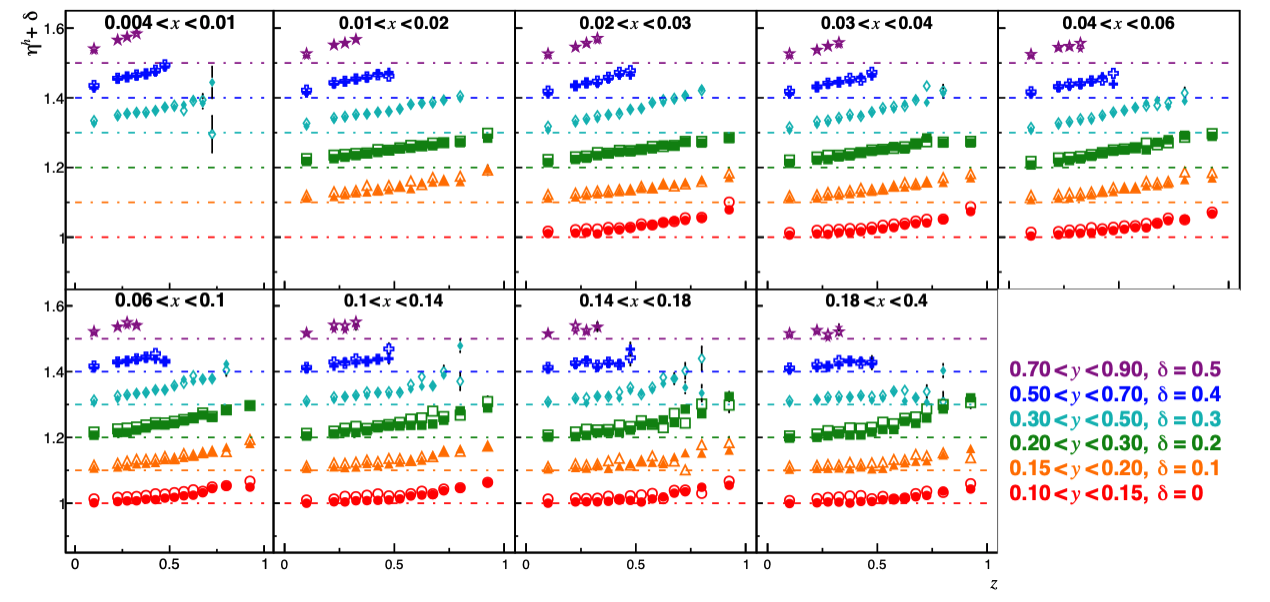
\includegraphics[scale=0.5]{./gfx/RadCor.png}
	\caption{Electron corrections (TBD)}
	\label{pic:ehad}
\end{figure}

\begin{figure}[!h]
	% 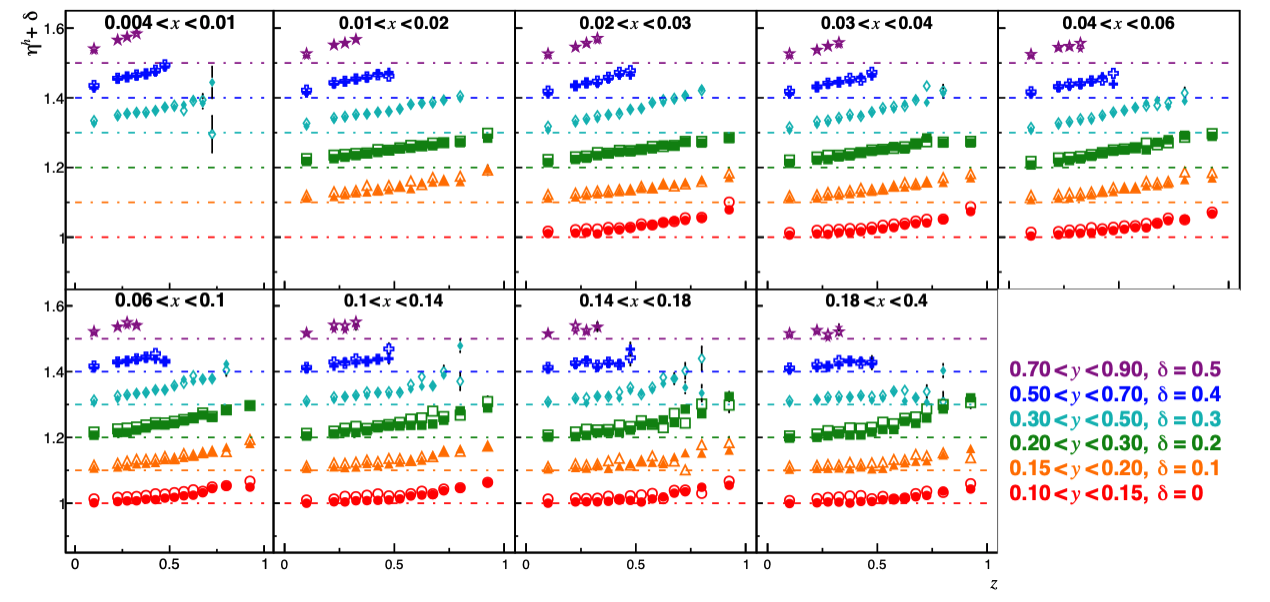
\includegraphics[scale=0.5]{./gfx/RadCor.png}
	\caption{Electron corrections (TBD)}
	\label{pic:epi}
\end{figure}

\section{Summary}

The most important correction is the acceptance $A(x,y,z)$, which accounts for the geometrical limitations of the apparatus, the data reconstruction efficiency and the detector efficiencies. This correction for charged hadrons is mostly of 70\% but can drop down to 30\% in some bins. The electron contamination correction, which corrects for the inability of the RICH to distinguish electrons and pions above 8 Gev/$v$, is embedded inside the acceptance correction.

The correction factor for the vector meson production $B^h(x,y,z)$ contaminating the hadron sample varies from 0 to 40\% at high $z$ for pions and 0 to 20\% at medium $z$ for kaons. This correction is model dependent.

The correction factor related to the radiative corrections, taking into account the discrepancy between hadronic and leptonic kinematic variable due to the emission of a real photon, hence biaising the kinematic distribution, is going from 0 to 20\%, the highest correction being located at high $y$ and high $z$.
